\chapter{Controller Development}

\section{Active Compliance}
Active vs. Passive Compliance
Passive compliance consists of using mechanical spring-damper components to adjust the dynamics of a robotics end effector. These come in the form of torsional springs, linear springs, hydraulic and pneumatic dampers to name a few. 

In the study by G.A. Pratt and M.M. Williamson  passive compliance in the form of a Series Elastic Actuator (SEA) was said to provide shock tolerance, lower reflected 
inertia, more accurate and stable force control, less damage to the environment, and the capacity for energy storage.\cite{Pratt1995}

Active compliance (AC) in robotic platforms is a relatively new area of research. Active compliance was chosen instead of passive compliance (PC) for the following reasons:

\begin{enumerate}
\item AC is mechanically simpler.
\item AC is mechanically lighter.
\item Good PC is expensive to implement due to lack of application specific off-the-shelf parts.
\end{enumerate}

Most importantly, AC can be configured on the fly to adapt to the environment of the robot. This allows a robot to, much like their biological equivalents, to comply to the environment based on various sensory inputs, or to perform various acrobatic tasks making use of spring-damper compression and decompression.

Various combinations of AC spring-damper configurations were designed, implemented and tested in order to determine the best topology.

\section{Dynamic Stability}
Stand still, look around, turn around - these apparently simple tasks are composed of a network of biologically advanced sensors and muscular motor movements that seem intuitive. To do the same relatively static and stable movement with a physically free robot is complex. 

The alternative to static stability is dynamic stability. Much like a spinning top remains stable due to gyroscopic effects when a stationary top topples over; a dynamically hopping leg remains upright with a relatively simple control system compared to a leg trying to remain upright and walk forward.

In the book by  M.H. Raibert et al., \textit{Legged Robots That Balance}, an easily adaptable simple control algorithm for dynamic legged hopping was published. ...

\section{Mechanical Impedance}
The leg design has inherent mechanical impedance in the form of friction, slack and inertial mass. Without mechanical impedance the leg would continue acting like an ideal system when actuated. This can be seen in \cref{sec:Virtual Spring-damper Tests} where the leg is modelled as a spring-damper - the amplitude of the oscillation of the virtual spring model with spring constant $K_s = 100$ decays with time. 

This mechanical impedance is not easily accounted for in the dynamic model of the leg as it is highly non-linear in the case of a complex linkage system as used in the Baleka leg - this makes it difficult to control. The mechanical impedance was treated as a disturbance and in the case of dynamic movement of the leg it was ignored. Energy will be lost in the hopping motion and during leg movement, but this is insignificant and only noticeable when doing spring-damper tests as seen in \cref{fig:spring-damper-tests}.

\section{Control Loop Sampling Frequency}

For high bandwidth proprioceptive force control S. Kalouche showed that the control loop sampling frequency should ideally be in the $kHz$ scale.\cite{Kalouche2016} This allows the foot force to ideally match the expected foot force when performing high frequency dynamic movements. 

The control loop sampling frequency was practically limited by the motor driver response time as seen in \cref{fig:packet-timing}. For every packet sent to the motor driver a response is required before the next packet can be sent otherwise the driver system becomes unstable. A maximum stable sampling frequency of $200 Hz$ was achieved with room for packet decoding, processing and controller action.

\section{Force Control}

\begin{figure}
\centering
\subfloat[][Caption]{
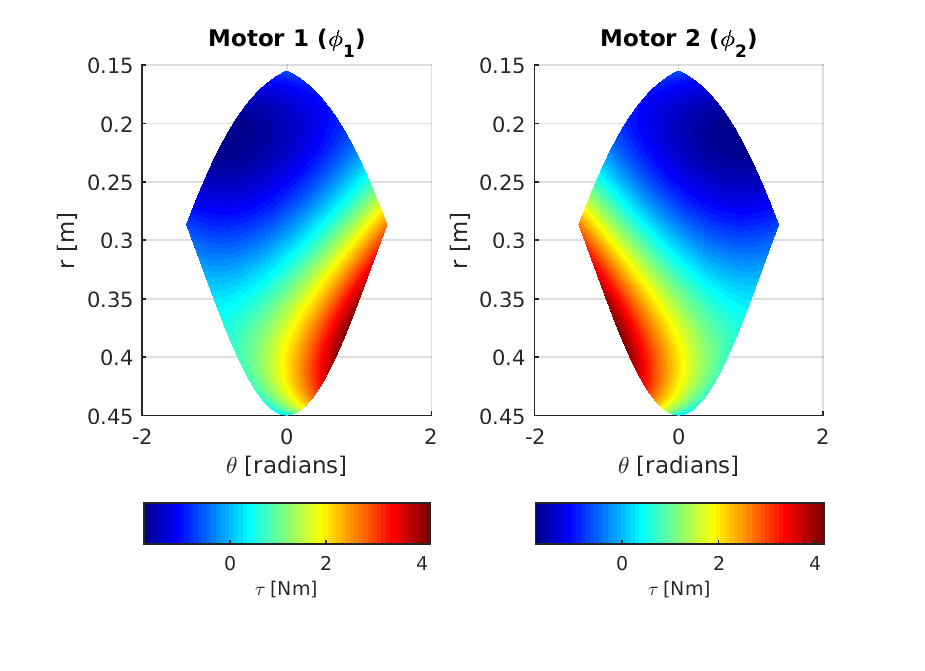
\includegraphics[width=0.8\textwidth]{images/control/forward-kinematic-motor-torque-s-0.eps} 
}

\subfloat[][Caption]{
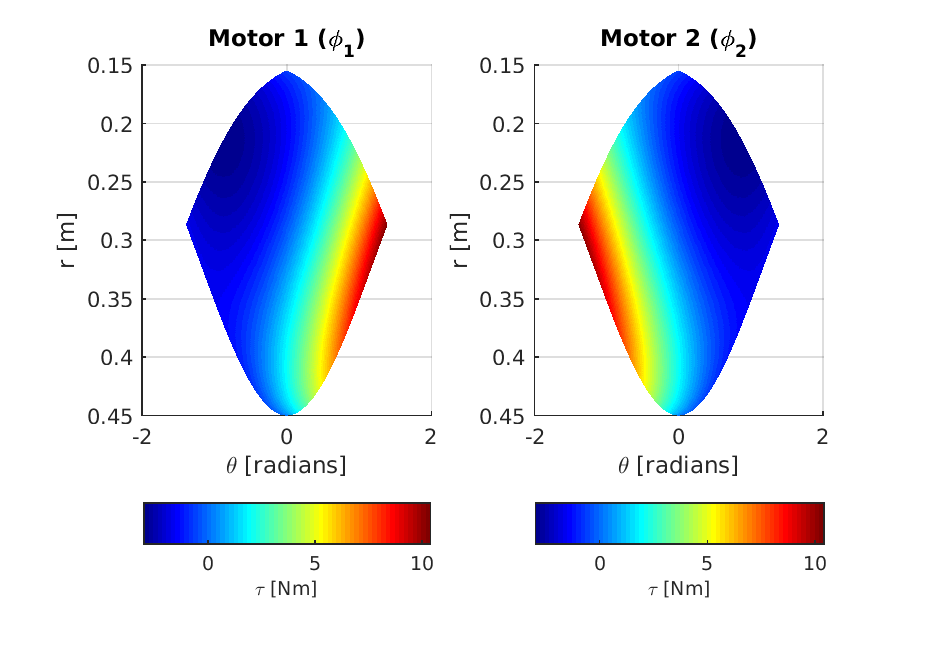
\includegraphics[width=0.8\textwidth]{images/control/forward-kinematic-motor-torque-theta-0.eps} 
}
\caption{Polar co-ordinate spring force mapping to motor torque.}
\label{fig:Polar co-ordinate spring force mapping to motor torque}
\end{figure}

\begin{figure}
\centering
\subfloat[][Caption]{
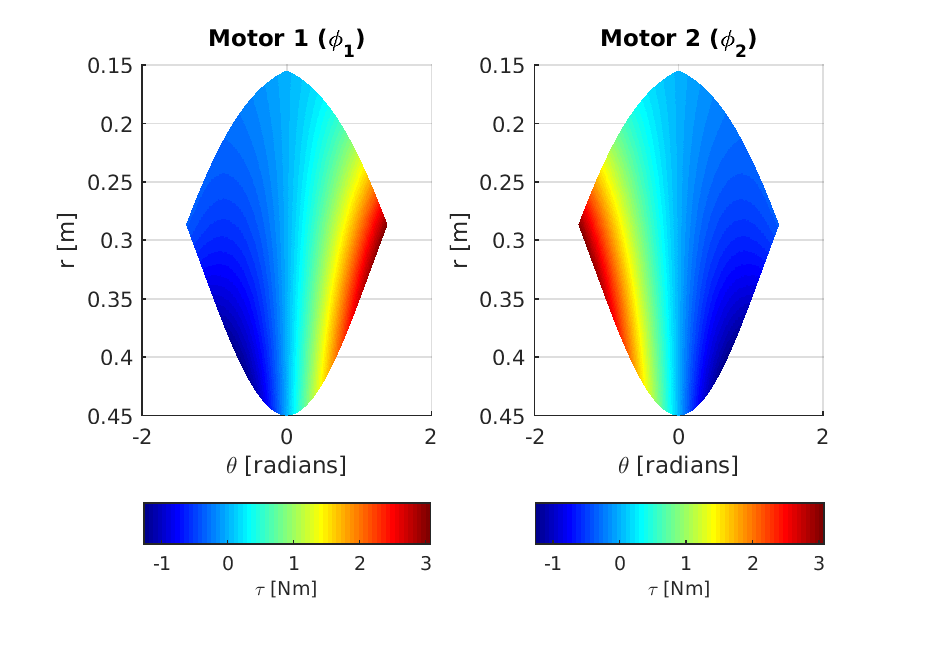
\includegraphics[width=0.8\textwidth]{images/control/forward-kinematic-motor-torque-s-only-0.eps} 
}

\subfloat[][Caption]{
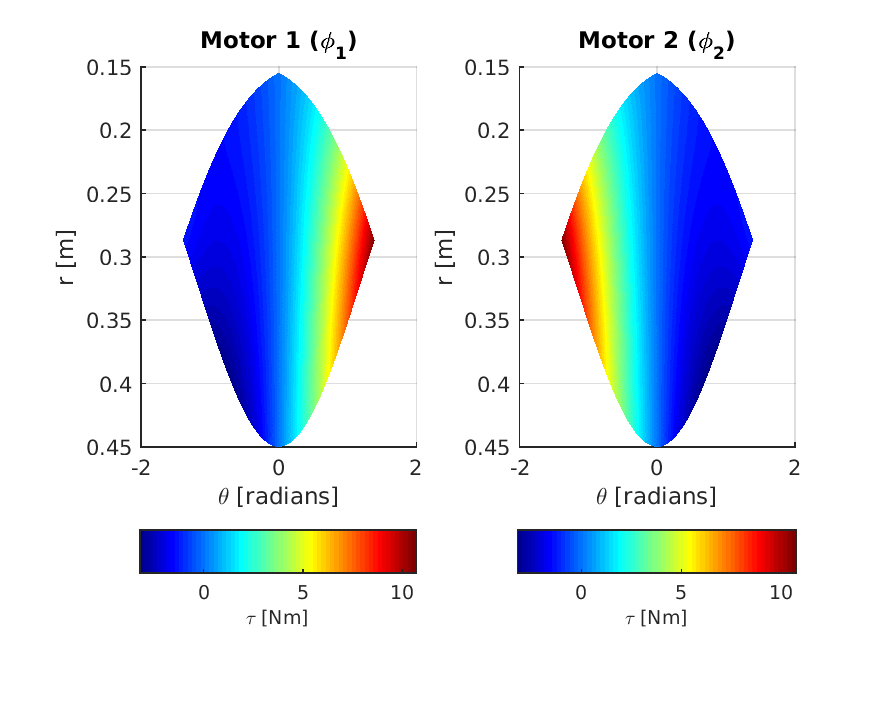
\includegraphics[width=0.8\textwidth]{images/control/forward-kinematic-motor-torque-theta-only-0.eps} 
}
\caption{Polar co-ordinate spring force mapping to motor torque.}
\label{fig:Polar co-ordinate spring force mapping to motor torque}
\end{figure}

\begin{equation}
\tau = J^TF
\end{equation}

\subsection{Current Control}


\section{Control Loop Design}
\Cref{fig:virtual-model-impedance-loop} is an adaptation of the control loop design found in \cite{Kalouche2016}. Continuous position loop gain scheduling vs virtual spring-damper gain scheduling.

\begin{figure}
\centering
\includegraphics[clip, trim=2cm 8cm 5cm 3cm, page = 1, width=1\textwidth]{images/control/virtual-model-impedance.pdf} 
\caption{Virtual model impedance control loop.}
\label{fig:virtual-model-impedance-loop}
\end{figure}

\subsection{Current Control for Impulse Launch}

Current saturation at 60A.

\subsection{Torsional Spring-damper}
$s = r \theta$\\

Normalises force - same unit of measurement, couples foot force to ground contact torque.

\begin{figure}
\centering
\includegraphics[width=1\textwidth]{images/control/theta-vs-arc.eps} 
\caption{Rotational foot force comparison using angle and arc-length torsional spring virtual model.}
\label{fig:Rotational foot force comparison}
\end{figure}

\subsection{Full-leg vs. Joint Active Compliance}